%%% LaTeX Template
%%% This template can be used for both articles and reports.
%%%
%%% Copyright: http://www.howtotex.com/
%%% Date: February 2011

%%% Preamble
\documentclass[paper=a4, fontsize=11pt]{scrartcl}	% Article class of KOMA-script with 11pt font and a4 format


\usepackage[italian]{babel}															% English language/hyphenation
\usepackage[protrusion=true,expansion=true]{microtype}				% Better typography
\usepackage{amsmath,amsfonts,amsthm}										% Math packages
\usepackage[pdftex]{graphicx}														% Enable pdflatex
%\usepackage{color,transparent}													% If you use color and/or transparency
\usepackage[hang, small,labelfont=bf,up,textfont=it,up]{caption}	% Custom captions under/above floats
\usepackage{epstopdf}																	% Converts .eps to .pdf
\usepackage{subfig}																		% Subfigures
\usepackage{booktabs}																	% Nicer tables
\usepackage[utf8x]{inputenc} 
\usepackage{listings}
\usepackage{xcolor}
\lstdefinestyle{sharpc}{language=[Sharp]C, frame=lr, rulecolor=\color{blue!80!black}}

  \usepackage{courier}

%%% Advanced verbatim environment
\usepackage{verbatim}
\usepackage{fancyvrb}
\DefineShortVerb{\|}								% delimiter to display inline verbatim text


%%% Custom sectioning (sectsty package)
\usepackage{sectsty}								% Custom sectioning (see below)
\allsectionsfont{%									% Change font of al section commands
	\usefont{OT1}{bch}{b}{n}%					% bch-b-n: CharterBT-Bold font
%	\hspace{15pt}%									% Uncomment for indentation
	}

\sectionfont{%										% Change font of \section command
	\usefont{OT1}{bch}{b}{n}%					% bch-b-n: CharterBT-Bold font
	\sectionrule{0pt}{0pt}{-5pt}{0.8pt}%	% Horizontal rule below section
	}


%%% Custom headers/footers (fancyhdr package)
\usepackage{fancyhdr}
\pagestyle{fancyplain}
\fancyhead{}														% No page header
\fancyfoot[C]{\thepage}										% Pagenumbering at center of footer
\renewcommand{\headrulewidth}{0pt}				% Remove header underlines
\renewcommand{\footrulewidth}{0pt}				% Remove footer underlines
\setlength{\headheight}{13.6pt}

%%% Equation and float numbering
\numberwithin{equation}{section}															% Equationnumbering: section.eq#
\numberwithin{figure}{section}																% Figurenumbering: section.fig#
\numberwithin{table}{section}																% Tablenumbering: section.tab#


\definecolor{pblue}{rgb}{0.13,0.13,1}
\definecolor{pgreen}{rgb}{0,0.5,0}
\definecolor{pred}{rgb}{0.9,0,0}
\definecolor{pgrey}{rgb}{0.46,0.45,0.48}


\usepackage{color}
\usepackage{xcolor}
\usepackage{listings}

 \lstset{
         basicstyle=\footnotesize\ttfamily, % Standardschrift
         %numbers=left,               % Ort der Zeilennummern
         numberstyle=\tiny,          % Stil der Zeilennummern
         %stepnumber=2,               % Abstand zwischen den Zeilennummern
         numbersep=5pt,              % Abstand der Nummern zum Text
         tabsize=2,                  % Groesse von Tabs
         extendedchars=true,         %
         breaklines=true,            % Zeilen werden Umgebrochen
         keywordstyle=\color{red},
    		frame=b,         
 %        keywordstyle=[1]\textbf,    % Stil der Keywords
 %        keywordstyle=[2]\textbf,    %
 %        keywordstyle=[3]\textbf,    %
 %        keywordstyle=[4]\textbf,   \sqrt{\sqrt{}} %
         stringstyle=\color{white}\ttfamily, % Farbe der String
         showspaces=false,           % Leerzeichen anzeigen ?
         showtabs=false,             % Tabs anzeigen ?
         xleftmargin=17pt,
         framexleftmargin=17pt,
         framexrightmargin=5pt,
         framexbottommargin=4pt,
         %backgroundcolor=\color{lightgray},
         showstringspaces=false      % Leerzeichen in Strings anzeigen ?        
 }
\lstloadlanguages{% Check Dokumentation for further languages ...
         %[Visual]Basic
         %Pascal
         %C
         %C++
         %XML
         %HTML
         %Java
{[Sharp]C}
 }
\usepackage{caption}
\DeclareCaptionFont{white}{\color{white}}
\DeclareCaptionFormat{listing}{\colorbox{gray}{\parbox{\textwidth}{#1#2#3}}}
\captionsetup[lstlisting]{format=listing,labelfont=white,textfont=white}

%%% Title	
\title{ \vspace{-1in} 	\usefont{OT1}{bch}{b}{n}
		\huge \strut Implementazione di Finding Triangles con Hadoop MapReduce\strut \\
		\Large \bfseries \strut Sistemi di elaborazione di grandi quantità di dati 2013 \strut
}
\author{ 									\usefont{OT1}{bch}{m}{n}
        Nicola Febbrari\\		\usefont{OT1}{bch}{m}{n}
        Università degli Studi di Verona\\	\usefont{OT1}{bch}{m}{n}
        Facoltà MM.FF.NN.\\
        \texttt{nicola.febbrari@studenti.univr.it}
}
\date{13 gennaio 2014}

%%% Begin document
\begin{document}
\maketitle
\section{Introduzione}
Lo scopo del progetto è quello di implementare un algoritmo per calcolare il numero di triangoli presenti in un grafo non diretto, utilizzando le tecniche di MapReduce e il Framework Haddop.


\section{Il problema}
I social network negli ultimi anni hanno avuto una notevole diffusione, l'aumento esponenziale del numero di utenti che interagistcono con questi sistemi 
ha avuto come diretta conseguenza un  incremento della quantità di dati che devono essere registrati, gestiti ed ovviamente elaborati.
Un social network può essere rappresentato matematicamente da un grafo e una caratteristica molto interessante di questo grafo e' il numero di 
triangoli\footnote{Dati 3 nodi (A,B,C) in un grafo, se un nodo A si relaziona sia con B che con C, nel grafo viene a formarsi un triangolo se esiste anche la relazione che lega B con C.} 
contenuti in sesso. 
Il numero di questi triangoli rapportato al numero totale di triangoli che esisterebbero con una distribuzione casuale e uniforme delle relazioni può essere un indice di quanto sia social il grafo analizzato.\\
\\
\\
\section{Strumenti e Framework}
Per progettare, implementare e testare il programma ho utilizzato:
\paragraph{Infrastruttura}
Per semplicità e rapidita di configurazione ho deciso di utilizzare Claudera come distribuzione di Hadoop nella sua versione per Docker.

\paragraph{Sviluppo}
Dovendo utilizzare il Framework Hadoop è il programma è stato scritto in Java utilizzando le API di Hadoop 2.6\\
L' IDE di sviluppo utilizzato è IntelliJ.  

\paragraph{Versioning}
Come sistema di versioning è stato utilizzato Git e GitHub come spazio di hosting dei files sorgenti.


\section{Implementazioni}
\subsection{Algoritmo 2 Jobs}
L'algoritmo a 2 Jobs prevede un prima fase in cui vengono elaborate tutte le relazioni e viene creata in output la combinazione di tutti i possibili triangoli a meno dell'ultimo arco necessario per chiudere il triangolo.\\
Esempio date le relazioni A - K, K - B e A - B  (in cui A<K<B ) il Job 1 elabora le relazioni in cui K è nodo in un caso maggiore o minore unendo queste relazioni trova al coppia A - B che verrà cercate nel Job2. Se questa relazione è presente allora esiste sicuramente il atriangolo A K B


\begin{figure}[h]
\centering
        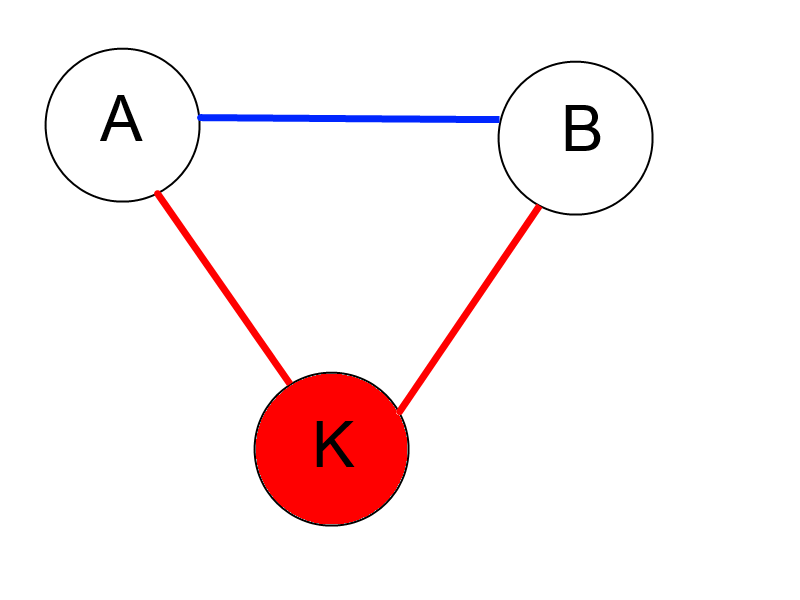
\includegraphics[totalheight=6cm]{Graph1.png}
    \caption{Il Job 1 elabora le relazioni rosse in cui K  in un caso è nodo  maggiore e nell altro caso minore. Il Job2 cerca la relazione blu A B.}
    \label{fig:verticalcell} 
\end{figure}
\paragraph{Job1 Mapper}
Nella parte di mapper del primo Job come prima cosa escludo tutti gli archi che portano nello stesso nodo e poi definisco le relazioni solamente come da nodo minore a nodo maggiore in modo da evitare duplicazioni. La definizione di triangolo in un grafo non prende in considerazione la direzione delle relazioni fra i nodi e nel mio caso i nodi sono rappresentati da dei valori Long, quindi la relazione di ordinamento è immediata.\\ 
In questa fase per ogni relazione mando in output 2 oggetti <<VALUE1,BOOL>,VALUE2>. Come KEY (<VALUE1,BOOL>) del VALUE (VALUE2) che passo al reducer uso un dato strutturato contenente il nodo e un valore booleano che identifica se il nodo VALUE è un nodo minore o maggiore di quello della KEY secondo la relazione di ordinamento definita. 

\lstset{
language=Java,
  showspaces=false,
  showtabs=false,
  breaklines=true,
  showstringspaces=false,
  breakatwhitespace=true,
  commentstyle=\color{pgreen},
  keywordstyle=\color{pblue},
  stringstyle=\color{pred},
  basicstyle=\ttfamily,
  moredelim=[il][\textcolor{pgrey}]{$$},
  moredelim=[is][\textcolor{pgrey}]{\%\%}{\%\%}
}
\begin{lstlisting}[label=Mapper1,caption=Implementazione del Mapper1]
@Override
	public void map(LongWritable key, Text value, Context context)
			throws IOException, InterruptedException {
		String line = value.toString();
		String[] sp = line.split("\s+");// splits on TAB
		Long lp0=Long.parseLong(sp[0]);
		Long lp1=Long.parseLong(sp[1]);
		if (lp0!= lp1) { 	//exclude self relation
			if (lp0 < lp1) {
				textP.set(lp1, false);
				text.set(lp0);
				context.write(textP, text);// "0" link_from
				textP.set(lp0, true);
				text.set(lp1);
				context.write(textP, text);// "1" link_to
			} else {
				textP.set(lp0, false);
				text.set(lp1);
				context.write(textP, text);// "0" link_from

				textP.set(lp1, true);
				text.set(lp0);
				context.write(textP, text);// "1" link_to
			}
		}
}\end{lstlisting}
\paragraph{Job1 Reducer}

Per suddividere correttamente tutti gli elementi prodotti dal Mapper sono stati ridefiniti il SortComparator e il GroupingComparator.
Il nuovo GroupingComparator ragruppa le chiavi valutando solamente il valore del nodo chiave K e garantendo che tutte le relazioni che contengono K come nodo maggiore o come nodo minore vengano elaborate dallo stesso reducer. Il SortComparator ridefinito invece ordina gli elementi in base al valore del nodo chiave K e in caso di uguale nodo chiave mette prima gli elementi con valore booleano false nella chiave.\\ Il reducer  garzie all'ordinamento esamina prima tutte le relazioni in cui il nodo chiave è nodo maggiore, queste coppie (nodo valore - nodo chiave) salvati in una lista L. Una volta che tutte le relazioni in cui il nodo chiave è nodo maggiore sono finite inizieranno le relazioni in cui il nodo chiave è nodo minore. Per ognuna di queste nuove relazioni (es. K-B) il reducer cicla la lista L mandando in output per ogni elemento (A-K) in L una relazione (A-B, K). Infatti la presenza della relazione A-B nel grafo chiuderebbe il triangolo A-K-B 

Il redoucer, grazie alla redifinizione del GroupinComparator1 (ragruppa le chiavi valutando solamente il valore del nodo della chiave) e  del Comparator1 (ordina le chiavi mettendo prima quelle con valore false ) tutti gli output del task di Map. Prima salva in una lista l'elenco dei nodi padre del nodo chiave, una volta che tutti i nodi sono stati ciclati, per ogni nodo figlio, scrive in output la terna di valori con la coppia nodo padre - nodo figlio che completerebbe il triangolo.
\begin{lstlisting}[label=Reducer1,caption=Implementazione del Reducer1]	
	@Override
	protected void reduce(LongBit key, Iterable<LongWritable> values, Context context)
			throws IOException, InterruptedException {
		partialJoin.clear();
		LongWritable k = key.getFirst();

		for (LongWritable valText : values) {
			Long val = valText.get();
			if (!key.getSecond().get())// link from
			{
				if (!partialJoin.contains(val))
					partialJoin.add(val);
			} else // link to
			{
				WriteContext(k, context, val);
			}
		}
	}
\end{lstlisting}
\paragraph{Job2 Mapper}
Nella secondo Job l'output del primo Job viene unito nuovamente alla sorgente dati iniziale. Il secondo mapper in questo scorre l'unione dei 2 input, nel caso la relazione è una relazione presente nel grafo iniziale scrive in output un elemento ((A,B,false),0) se invece è generata dal Job 1 scrive in output  ((A,B,true),K) dove A,B sono nodi della relazione e K è nodo intermedio fra A e B calcolato da Job1.
\paragraph{Job2 Reducer}
Il secondo reducer ridefinendo in modo analogo al Reducer1 una seconda versione del SortComparator e del GroupingComparator, scorre l'input prima cerca le relazioni AB che chiuderebbero un triangolo e poi per ogni relazione generata dal Job1 con output AB manda in output AKB.
Questo algoritmo se dal punto di vista implementativo è stato estremamente semplice tuttavia testato con grafi ad elevato numero di nodi e con una grande densità di triangoli  si è rilevatoinefficiente.



\subsection{Algoritmo 4 Jobs}
L'algoritmo a 4 Jobs prevede prima una fase in cui i primi 2 Jobs costuiscono una struttura dati che poi verrà usata negli ultimi 2 Jobs, i quali andranno ad eseguire il calcolo dei triangoli.
\paragraph{Job 1}
Il primo Job è molto semplice e per ogni arco emette un valore 1. Il redoucer conta tutti questi valori, ne fa la somma che poi scrive come output.
\paragraph{Job 2}
Il mapper del secondo Job per ogni arco (A,B) emette 2 valori (A 1 e B 1) un per ogni nodo che compone (A,B).\\
Le funzioni di grouping e il partitioner mi garantiscono che tutti i valori di uno stesso nodo vengono accumulati nello stesso redoucer e nello stesso ciclo iterativo. Completato il ciclo scrive in output per ogni nodo la somma di tutti i valori emessi dal mapper. Questo valore rappresenta il grado del nodo.
\paragraph{Job 3}
Nella seconda fase viene eseguito l'algoritmo vero e proprio.\\
Nel Job 3 l'algoritmo estrapola tutti quei triangoli che sono composti da nodi Heavy Hitter, ovvero con un grado maggiore alla radice di m dove m è il numero degli archi delgrafo.
Il mapper utilizzando il lavoro dei Jobs precedenti costruisce un indice con i gradi di ogni nodo e successuvamente elimina dall'analisi tutti i nodi non HH.\\
Con questo sottografo costruisce una suddivisione delle relazioni definendo delle chiavi strutturate e abbinate ai vari task di Reduce. Questa suddivisione viene realizzata definendo una funzione Hash sul valore del nodo stesso.\\
Come prima cosa viene definita una relazione di ordinamento dei nodi in base al grado.
Ogni trinagolo è formato da  3 nodi (x,y,z) i quali sono legati dalle 3 relazioni typeA=(x,y) con x\lly, typeB=(x,z) con x\llz e typeC=(y,z) ocn y\llz. Ogni relazione presente nel grafo può essre una delle 3 che compongono il triangolo, quindi dato R=(u,v), R può essere una relazione typeA e quindi  il triangolo sarebbe (u,v,?) oppure typeB con (u,?,v) o typeC con (?,u,v).
Il task di Map per sfruttare il parallelismo dei redoucer divide le relazioni in tante parti quante le possibili casistiche in cui la relazione può essere utilizzata per completare un triangolo.\\
Per implementare questa suddivisione, come prima cosa, viene definito un paramentro b che indica quanti sono i possibili valori in output della funzione hash. In base a questo parametro ogni relazione di input R(x,y) viene distribuita nei rispettivi 3bk Reducers utilizzando la funzione di hash h e seguendo questo schema: (h(x),h(y),1\lei\llb) impotizzando che R sia di tipo A , (h(x),1\lei\leb,h(y)) se R fosse di tipo B e (1\lei\leb,h(x),h(y)) se R fosse di tipo C. Ogni relazione R viene inclusa in tutti i possibili reducer in cui potrebbe essere utilizzata per il completamento di un triangolo.
Il reducer, doppo una opportuna ridefinizione delle classi di Gruouping e Ordinamento, scorrere tutti gli elementi in input. L'ordinamente è definito in modo da analizzare, per ogni nodo a, prima le possili relazioni di tipo A, per ognuna di esse viene inserito il nodo destinazione b in una Lista LAa. Successivamente vengono analizzate le relazioni di a di tipo B con c come nodo di destinazione, per ognuna di esse viene preso creata una Map in cui la chiave è la copia formata da ogni elemento di Laa e c e il valore è il nodo a.
L'analisi successiva della relazione di tipo C fra a e d, se nella Map esiste una chiave formata dalla coppia a,d con valore e allora nel grafo esisterà un triangolo e,a,d.
L'ordinamento con cui viene eseguita questa analisi consente di ottimizzare lo spazio di memoria utilizzato e ci garantisce che ogni triangolo viene rilevato solo una volta.
\paragraph{Job 4}
Il Job 4 è molto simile al Job3 l'unica differenze è che in questo caso si volgiono escludere tutti i triangoli di tipo HH.\\
Data una relazione x,y se x è HH x,y potrebbe appartenere ad un triangolo non HH se solo se x,y è di tipo C. Infatti per la relazione di ordinamento rel definita precedentemente dato il triangolo T1(x,y,?) in cui x,y è di tipo A, qualsiasi ? e y sarebbero maggiori di x e quidi T1 sarebbe HH, la stessa cosa se x,y fosse di tipo B.\\
Grazie a questa caratteristica il mapper esclude le relazioni di tipo A e B in cui x,y ha x HH.
Il reducer è lo stesso del Job4.


\section{Valutazioni}
\paragraph{Algoritmo 2 Jobs}
Semplice ma ha evidenziato problemi analizzando grafi di grandi dimensioni. 
\paragraph{Algoritmo 4 Jobs}
Più complesso ottimizzato dal punto di vista del tempo, tuttavia presenta sempre dei problemi nell'utilizzo della memoria. Sicuramente è possibile fare delle ottimizzazioni utilizzando delle strutture dati di opportune.\\ 
Nella mia implementazione ho cercato di utilizzare le strutture dati che mi permettevano di avere tempi di accesso rapidi e che non utlizzassero troppa memoria. Purtroppo ho notato che eseuendo più volte il programma rimane allocata della memoria, questo mi fa presupporre che vi sono alcuni memory leak.\\

\section{Sviluppi futuri}
Oltre alle ottimizzazioni nell'utilizzo di strutture dati più performanti, mi sarebbe piaciuto generare come artefatto del processo un immagine dock pronta all'uso. Sarebbe interessante provare a fare un deploy per testare questo container in un ambiente cloud che supporta Docker.

\end{document}